\chapter{Implementation and Assessment}
\label{chp:Implementation_and_Assessment}

All algorithms discussed in this work are realized in \mbox{MATLAB}, a programming language specialized on matrix manipulations.
It is especially useful for high-dimensional matrix operations, such as the ones for this work.
The following text explains the implementation of the theoretical models and concepts discussed in the previous chapters.
For the implementation, the goal was to make the pipeline as flexible as possible to support all kinds of light fields in different formats.

\section{Requirements}
\label{sec:requirements}

For the implementation and physical realization, some assumptions and requirements have to be formulated.
The input light field for the optimization algorithm is expected to be a five dimensional array $L$ with entries $L_{ijklc}$, where pairs $(i, j)$ and $(k, l)$ correspond to the angular- and spatial coordinates, and $c$ indexes the color channel. 
The data is normalized such that $L_{ijklc} \in \left[0, 1\right]$.
It is also assumed that the light field is rectified such that indices $i, j$ conform to global coordinates on the $(s, t)$-plane as explained in section~\ref{sec:light_field_aquisition}.
In addition, the baseline as well as the distance between the two planes are a required input for the system.

The attenuator is defined by the number of layers, resolution, size and thickness.
Each layer has the same dimensions and resolution and is modeled to be infinitely thin.
Also, the backlight is modeled as a constant white light field, $L_0 \equiv 1$.

\section{The Basic Procedure}
\label{sec:basic_procedure}

As described in section~\ref{sec:ray_casting}, the two virtual planes that parameterize the light field are placed relative to the attenuator and by ray casting, the entries of the propagation matrix $P$ are computed.
Next, the constrained optimization problem given in equation~\ref{eq:minimize_norm} is solved independently for each color channel using an iterative solver of choice, e.g. \mbox{SART}.
The outcome of each optimization is a vector $\alpha_c$ containing the attenuation values in the interval $\left[ 0, \infty \right)$ where $c = 1, 2, 3$ (red, green, blue) denotes the color channel.
The transmittance values are then obtained by element-wise exponentiation, $t = \exp(-\alpha)$, which holds values between zero and one.
Finally, the linearly indexed vector $t$ is reshaped so that the layers can be extracted as three-dimensional matrices and printed on transparencies.

In order to evaluate the attenuation masks, one has to compare the emitted light field $L^\ast = \exp(- P \alpha)$ with the original, $L$.
For instance, one could evaluate the squared 2-norm of the difference $L - L^\ast$ in each color channel.
However, this resulting number is not very meaningful because it also varies with the size of the light field, i.e. the angular and spatial resolution.
This makes it harder to compare the display quality between different light fields.
Thus, it is better to use a normalized figure such as the mean squared error \mbox{(MSE)} or the root-mean-square error \mbox{(RMSE)} defined as
\begin{equation*}
	\text{MSE} \coloneqq \frac{1}{n} \sum_{i = 1}^{n} (X - X^\ast)^2 = \frac{1}{n} \lVert X - X^\ast \rVert^2
	\quad \text{and} \quad
	\text{RMSE} \coloneqq \sqrt{\text{MSE}}
\end{equation*}
for vectors $X, X^\ast \in \mathbb{R}^n$.
To deal with the color channels, the \mbox{MSE} is computed for each color component and then averaged.
Another important quality measure in signal processing is the peak signal-to-noise ratio \mbox{(PSNR)} defined as
\begin{equation*}
	\text{PSNR} \coloneqq 10 \log_{10} \left(\frac{X_\text{max}^2}{\text{MSE}}\right),
\end{equation*}
where $X_\text{max}$ is the maximum intensity value the image or color channel can hold, e.g. for 8-bit color channel representation this value would be 255.
It measures the loss of power in a reconstructed signal, with an additional adjustment for the human perception of error.
The use of this measure is motivated by the fact that \mbox{Layered 3D} is also about signal reconstruction, and the goal is to compare the original signal (light field) with the reconstructed one. 
As opposed to the MSE, it is easier to compare the PSNR of different images because it does not depend on the pixels intensity scale given by the bit depth.
Generally, a higher \mbox{PSNR} indicates greater image fidelity and conversely, a highly corrupted signal produces low \mbox{PSNR}.

The following sections present a variety of ideas and improvements that were implemented on top of the standard procedure explained above.
Next to that, the results are evaluated using the introduced error measures.

\section{Challenges with Ray Casting}
\label{sec:challenges_ray_casting}

In section~\ref{sec:ray_casting} it was explained how to compute the pixel indices on the layers for a ray that passes the attenuator.
But it is not entirely obvious how to sample the rays in the first place.
One of the simplest methods is to cast one ray per image pixel for each of the virtual cameras as it is illustrated in figure~\ref{fig:ray_casting_from_camera}. 
\begin{figure}[tb]
	\subcaptionbox{\label{fig:ray_casting_from_camera}}{\documentclass[tikz]{standalone}

\usetikzlibrary{intersections}

\begin{document}
	\begin{tikzpicture}[scale = 0.5, baseline, rotate = -90]
		
		\begin{scope}
			\clip (0, 5.5) rectangle (6, -5.5);
		
			% Back-projection volume of pixels
			\fill[fill opacity = 0.1, fill = blue] (0, 0) -- ({atan(3 * tan(30) / 2)} : 12cm) -- ({atan(1 * tan(30) / 2)} : 12cm) -- (0, 0);
			\fill[fill opacity = 0.1, fill = yellow] (0, 0) -- ({atan(1 * tan(30) / 2)} : 12cm) -- ({atan(-1 * tan(30) / 2)} : 12cm) -- (0, 0);
			\fill[fill opacity = 0.1, fill = red] (0, 0) -- ({atan(-1 * tan(30) / 2)} : 12cm) -- ({atan(-3 * tan(30) / 2)} : 12cm) -- (0, 0);
		\end{scope}
	
		% Three rays from camera
		\draw[name path = ray1, ->] (0, 0) -- (30 : 8cm);
		\draw[name path = ray2, ->] (0, 0) -- (0 : {cos(30)*8}cm);
		\draw[name path = ray3, ->] (0, 0) -- (-30 : 8cm);
		
		% Center of projection
		\fill (0, 0) circle[radius = 0.1] node[right] {Camera};
		
		% Image plane
		\draw[name path = imagePlane, ->] (2, -3) -- (2, 3) node[right] {$s$};
		
		% Pixel markers on image plane
		\draw (2, {3 * tan(30) * 2 / 2}) -- ++(0.2, 0) -- ++(-0.4, 0);
		\draw (2, {tan(30) * 2 / 2}) -- ++(0.2, 0) -- ++(-0.4, 0);
		\draw (2, {-tan(30) * 2 / 2}) -- ++(0.2, 0) -- ++(-0.4, 0);
		\draw (2, {-3 * tan(30) * 2 / 2}) -- ++(0.2, 0) -- ++(-0.4, 0);
		
		% Layer axis
		\draw[name path = layer1, <-] (4.5, 5.5) -- (4.5, -5.5) node[pos = 0.05, anchor = south west, above] {Layer 2};
		\draw[name path = layer2, <-] (6, 5.5) -- (6, -5.5) node[pos = 0.05, anchor = south west, above] {Layer 1};
		
		% Layer set of pixels
		\foreach \x in {1,...,10} 
			\draw (4.5, 10 / 2 * 1 - \x * 1 + 0.3) -- ++(0.2, 0) -- ++(-0.4, 0);
		
		\foreach \x in {1,...,10} 
			\draw (5 + 1, 10 / 2 * 1 - \x * 1 + 0.3) -- ++(0.2, 0) -- ++(-0.4, 0);
		
		% Dots at intersections on image plane
		\fill[name intersections={of=imagePlane and ray1, total=\t}, blue]
			\foreach \s in {1,...,\t}{(intersection-\s) circle[radius = 0.15]};
			
		\fill[name intersections={of=imagePlane and ray2, total=\t}, blue]
			\foreach \s in {1,...,\t}{(intersection-\s) circle[radius = 0.15]};
		
		\fill[name intersections={of=imagePlane and ray3, total=\t}, blue]
			\foreach \s in {1,...,\t}{(intersection-\s) circle[radius = 0.15]};
		
		% Dots at intersections on first layer
		\fill[name intersections={of=layer1 and ray1, total=\t}, red]
			\foreach \s in {1,...,\t}{(intersection-\s) circle[radius = 0.15]};
		
		\fill[name intersections={of=layer1 and ray2, total=\t}, red]
			\foreach \s in {1,...,\t}{(intersection-\s) circle[radius = 0.15]};
		
		\fill[name intersections={of=layer1 and ray3, total=\t}, red]
			\foreach \s in {1,...,\t}{(intersection-\s) circle[radius = 0.15]};
		
		% Dots at intersections on second layer
		\fill[name intersections={of=layer2 and ray1, total=\t}, red]
			\foreach \s in {1,...,\t}{(intersection-\s) circle[radius = 0.15]};
		
		\fill[name intersections={of=layer2 and ray2, total=\t}, red]
			\foreach \s in {1,...,\t}{(intersection-\s) circle[radius = 0.15]};
		
		\fill[name intersections={of=layer2 and ray3, total=\t}, red]
			\foreach \s in {1,...,\t}{(intersection-\s) circle[radius = 0.15]};
		
	\end{tikzpicture}
\end{document}
}\hfill %
	\subcaptionbox{\label{fig:interpolation_on_layers}}{\documentclass[tikz]{standalone}

\usetikzlibrary{intersections}

\begin{document}
	\begin{tikzpicture}[scale = 0.35, baseline]
		
		% First layer axis
		\draw[name path = layer1, ->] (-1, 3) --(11, 3) node[right] {Layer 2};
		
		% Second layer axis
		\draw[name path = layer2, ->] (-1, -1) --(11, -1) node[right] {Layer 1};
		
		% Pixel boundaries on first layer
		\foreach \i in {1,...,4} 
			\draw ({(\i - 1) * 3}, 3) -- ++(0, 0.5) -- ++(0, -1);

		% Pixel boundaries on second layer
		\foreach \i in {1,...,4} 
			\draw ({(\i - 1) * 3}, -1) -- ++(0, 0.5) -- ++(0, -1);	
			
		% Pixel centers on first layer	
		\foreach \i in {1,...,3} 
			\fill ({1.5 + (\i - 1) * 3}, 3) circle[radius = 0.2];	
		
		% Pixel centers on second layer	
		\foreach \i in {1,...,3} 
			\fill ({1.5 + (\i - 1) * 3}, -1) circle[radius = 0.2];	
			
		% The ray passing the two layers
		\begin{scope}
			\clip (0, 5) rectangle (11, -3);
			\coordinate (anchor) at (2.3, -1);
			
			\draw[name path = ray, red] (anchor) -- ++(46 : 10cm);
			\draw[red, ->] (anchor) -- ++(180 + 46 : 2cm);
		\end{scope}
		
		% Mark intersections with layers
		\fill[red] (anchor) circle[radius = 0.2];
		\fill[name intersections={of=layer1 and ray, total=\t}, red]
			\foreach \s in {1,...,\t}{(intersection-\s) circle[radius = 0.2]};
			
		% Interpolation markers and labels on first layer
		\draw[name intersections={of=layer1 and ray, total=\t}, blue, |-|]
			(intersection-1) ++(0, -1) -- node[below, yshift = -1.5] {$1 - \gamma_1$} (7.5, 2);
		
		\draw[name intersections={of=layer1 and ray, total=\t}, blue, |-|]
			(intersection-1) ++(0, 1) -- node[above, yshift = 1.5] {$\gamma_1$} (4.5, 4);
			
		% Interpolation markers and labels on second layer
		\draw[blue, |-|]
			(anchor) ++(0, 1) -- node[above, yshift = 1.5] {$\gamma_2$} (1.5, 0);
				
		\draw[blue, |-|]
			(anchor) ++(0, -1) -- node[below, yshift = -1.5] {$1 - \gamma_2$} (4.5, -2);
		
	\end{tikzpicture}
\end{document}
}
	\caption[Intersecting light rays with attenuation layers]
			{Intersecting light rays with attenuation layers.
			 (a) Alternative ray casting method. 
			 	 The rays are cast from the camera center through the pixel centers (blue) and intersect with the pixels on the layers (red).
			 	 The colored areas indicate the projection volume of an individual pixel on the image plane.
			 (b) Linear interpolation of the intersections between adjacent pixel centers marked by the black dots.}
\end{figure}
The sketch shows a one-dimensional pinhole camera with three pixels of equal width and the associated projection volumes.
Because of the perspective projection it is possible that multiple pixel elements on the layers project to a single pixel on the image plane.
If the strategy is to only cast one ray per image pixel, many layer pixels inside the respective projection volume are missed and thereby left unconstrained.
But precisely because they lie in the same projection volume, the missed pixels are equally important and should be considered when setting up the linear system of equations.
Note that although the proportions in the illustration are different for real-world applications, the problem exists in any case and the severity of it mainly depends on the resolution and placement of the layers. 

Based on this observation, it seems natural to sample more than one ray per camera pixel.
But then, how many rays are necessary? 
Again, because of the perspective projection, a uniform sampling of the image plane does not imply a uniform distribution of intersections on the layers.

\section{Interpolation}
\label{sec:interpolation}

In addition to nearest neighbor interpolation indicated in equation~\ref{eq:pixel_shift_perspective_projection}, bilinear interpolation is incorporated into the pipeline in order to reduce artifacts.
For every ray, the value of the intersection point on the attenuation layer is represented as a linearly weighted sum of four neighboring pixels corresponding to the rounded indices.
Accordingly, instead of storing $N$ binary weights, each row of the propagation matrix now holds $4 N$ values.
Essentially, this just means that each ray in the log-light field is a linear combination of $4 N$ absorbance values.
Due to the exponential propagation model, the interpolation in the log-domain translates to a multiplication of the transmittance simply by the exponential law,
\begin{equation*}	
	\exp( \gamma \alpha_i + (1 - \gamma) \alpha_j ) = \exp( \gamma \alpha_i ) \exp( (1 - \gamma) \alpha_j ) = t_i^{\gamma} t_j^{1 - \gamma},
\end{equation*}
with $\gamma$ being the linear interpolation weight, $i$ and $j$ identifying the neighboring pixels which are the query points for the interpolation.

The attempt of interpolation does not exhibit a significant increase in reconstruction quality.
Alternatively, interpolation could be applied to the transmittance instead of the absorbance, but this requires a different optimization strategy.
Because of the non-linearity of the logarithm, the optimization problem can not simply be transformed into a linear equation.

In general, it is not entirely clear which interpolation strategy one should choose for such a problem.
The choice depends on a variety of physical factors as well as implementation specific restrictions.
For example, an ink-jet printer produces slightly different attenuation masks than a laser printer.
One could estimate the point spread function (PSF) of the printer by observing the distribution of a single ink drop on the surface.
The interpolation weights should then be chosen according to the PSF.
This approach would take into account the very physical aspects of printing.
However, an accurate validation of this idea would introduce a lot of challenges because it requires accurate calibration and fabrication in order to compare the input light field with the displayed light field:
The measuring process would require two iterations, one with PSF interpolation and one without.
The attenuation layers need to be precisely aligned and placed in front of the capturing device (camera array, plenoptic camera etc.) such that the emitted light rays directly correspond to the original light rays.

\section{Oversampling}
\label{sec:oversampling}

Because of the perspective projection, all points that project to the camera's image plane are inside a pyramidal frustum.
Conversely, the area of a single pixel back-projects to a larger area on the original surface, or in this case, the attenuation layers.
This means that, depending on the resolution and size of the attenuator, the beam of light rays going through a single pixel on the image plane (\mbox{$(s,t)$-plane}) possibly covers multiple pixels on some of the attenuation layers.
This leads to fewer constraints on the layer pixels for the optimization when sampling only a single ray per image pixel.
The obvious solution would be to simply increase the resolution of the layers, but this is sometimes not feasible or desired due to the much longer runtime of the solver.
Instead, the sampling density can be increased while keeping the layer resolution the same.
In the current implementation, the sampling density can be controlled by a plane parallel to the attenuator.
Placing this sampling plane at the same location as the bottom-most layer (farthest from the camera) ensures that the ray-density is no smaller on the other layers.
Because the rays that are cast from the sampling plane to the image plane are different from the original rays, the light field is resampled to a higher resolution which also requires interpolation.

\section{Baseline Scaling and Back Projection}
\label{sec:baseline_scaling}

Often it is the case that the light field of interest has a depth range that does not match the depth of field of the display because of its fixed thickness.
As a consequence, objects outside the depth of field appear blurry as demonstrated in figure~\ref{fig:reconstruction_baseline_unscaled}
\begin{figure}[tb]
	\begin{subfigure}{0.5\textwidth}
		\centering
		\documentclass{standalone}
\usepackage{tikz}
\usetikzlibrary{intersections}

\begin{document}
	\begin{tikzpicture}[line width = 0.3mm]
	
	\node[anchor = center, inner sep = 0, outer sep = 0] (I) at (0, 0) {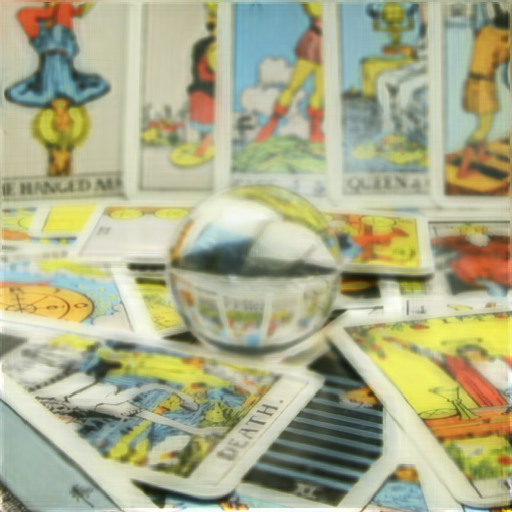
\includegraphics[width = 3.75cm]{../Figures/depth_compression/baseline_unscaled/Reconstruction_of_view_(9,9).png}};
	
	\coordinate (A1) at (-0.6, -1.7);
	\coordinate (S1) at (1, 1);
	\coordinate (A2) at (-1.7, 0.2);
	\coordinate (S2) at (1, 1);
	
	\draw[red]  (A1) rectangle ++(S1); 	
	\draw[blue] (A2) rectangle ++(S2); 
	
	% Magnification box 1
	\node[anchor = south west, xshift = 0.1cm, inner sep = 0pt, outer sep = 0pt, scale = 1.825] (box1) at (I.south east) {
		
		\begin{tikzpicture}
			\begin{scope}
				\clip(A1) rectangle ++(S1);
				\node[anchor = center, inner sep = 0pt] (I) at (0, 0) {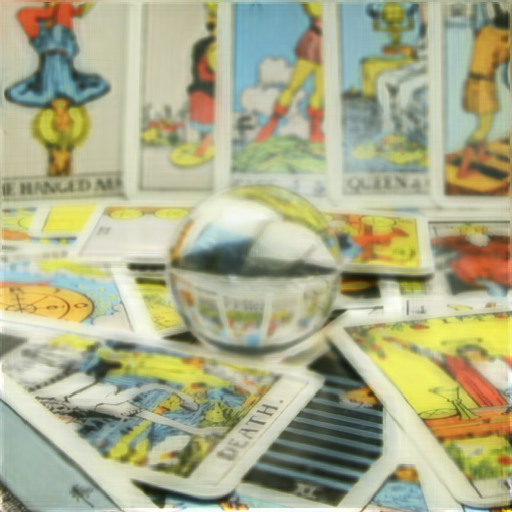
\includegraphics[width = 3.75cm]{../Figures/depth_compression/baseline_unscaled/Reconstruction_of_view_(9,9).png}};
			\end{scope}	
		\end{tikzpicture}
	};
	\draw[red] (box1.south east) rectangle (box1.north west);
	
	% Magnification box 2
	\node[anchor = north west, xshift = 0.1cm, inner sep = 0pt, outer sep = 0pt, scale = 1.825] (box2) at (I.north east) {
		
		\begin{tikzpicture}
			\begin{scope}
				\clip(A2) rectangle ++(S2);
				\node[anchor = center, inner sep = 0pt] (I) at (0, 0) {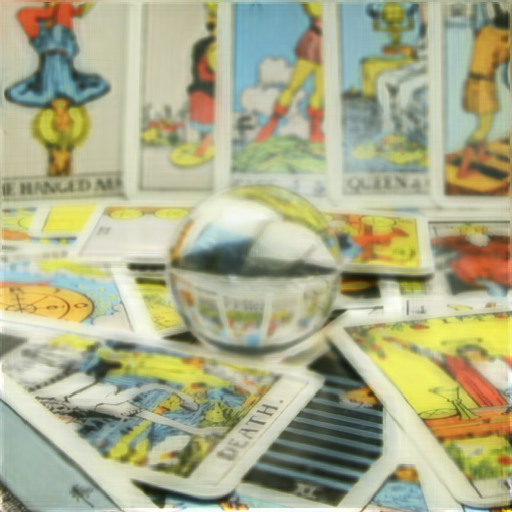
\includegraphics[width = 3.75cm]{../Figures/depth_compression/baseline_unscaled/Reconstruction_of_view_(9,9).png}};
			\end{scope}	
		\end{tikzpicture}
	};
	\draw[blue] (box2.south east) rectangle (box2.north west);
			
	
	\end{tikzpicture}
\end{document}

		\caption{}
		\label{fig:reconstruction_baseline_unscaled}
	\end{subfigure}%
	\begin{subfigure}{0.5\textwidth}
		\centering
		\documentclass{standalone}
\usepackage{tikz}
\usetikzlibrary{intersections}

\begin{document}
	\begin{tikzpicture}[line width = 0.3mm]
	
	\node[anchor = center, inner sep = 0, outer sep = 0] (I) at (0, 0) {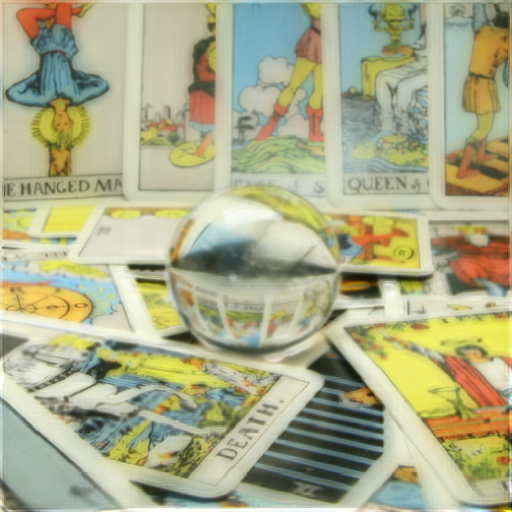
\includegraphics[width = 3.75cm]{../Figures/depth_compression/baseline_scaled_shifted/Reconstruction_of_view_(9,9).png}};
	
	\coordinate (A1) at (-0.6, -1.7);
	\coordinate (S1) at (1, 1);
	\coordinate (A2) at (-1.7, 0.2);
	\coordinate (S2) at (1, 1);
	
	\draw[red]  (A1) rectangle ++(S1); 	
	\draw[blue] (A2) rectangle ++(S2); 
	
	% Magnification box 1
	\node[anchor = south west, xshift = 0.1cm, inner sep = 0pt, outer sep = 0pt, scale = 1.825] (box1) at (I.south east) {
		
		\begin{tikzpicture}
			\begin{scope}
				\clip(A1) rectangle ++(S1);
				\node[anchor = center, inner sep = 0pt] (I) at (0, 0) {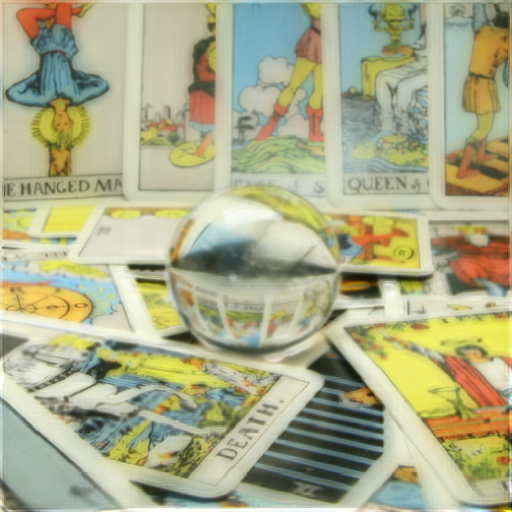
\includegraphics[width = 3.75cm]{../Figures/depth_compression/baseline_scaled_shifted/Reconstruction_of_view_(9,9).png}};
			\end{scope}	
		\end{tikzpicture}
	};
	\draw[red] (box1.south east) rectangle (box1.north west);
	
	% Magnification box 2
	\node[anchor = north west, xshift = 0.1cm, inner sep = 0pt, outer sep = 0pt, scale = 1.825] (box2) at (I.north east) {
		
		\begin{tikzpicture}
			\begin{scope}
				\clip(A2) rectangle ++(S2);
				\node[anchor = center, inner sep = 0pt] (I) at (0, 0) {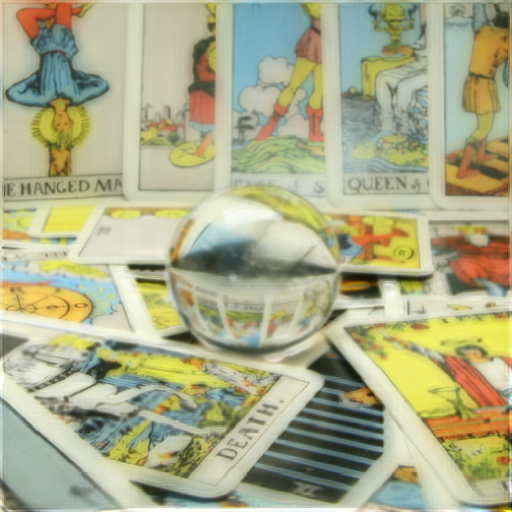
\includegraphics[width = 3.75cm]{../Figures/depth_compression/baseline_scaled_shifted/Reconstruction_of_view_(9,9).png}};
			\end{scope}	
		\end{tikzpicture}
	};
	\draw[blue] (box2.south east) rectangle (box2.north west);
			
	
	\end{tikzpicture}
\end{document}

		\caption{}
		\label{fig:reconstruction_baseline_scaled_shifted}
	\end{subfigure}
	\caption[Baseline scaling]
			{Depth compression by means of baseline scaling.
			 Shown is the reconstructed central angular view without proper baseline scaling (a) and with scaling (b).
			 The light field used here is from the Stanford light field archive, \mbox{\url{http://lightfield.stanford.edu}}.}
	\label{fig:baseline_scaling}
\end{figure}
The reconstruction shows that cards in the front and back are blurred because they are virtually further away from the display, while the objects in the center are sharper.
This problem can be solved by virtually scaling the baseline while keeping all other distances the same.
The effect is that depth is compressed and hence objects appear to be squeezed in Z-direction.
But the question is: How should one chose the scale such that a desired range is sharp?
It is possible to solve this problem analytically, for example by using equation~\ref{eq:approx_upper_bound_spatial_cut_off} or ~\ref{eq:expected_upper_bound_spatial_cut_off}.
But often it is the case that the exact baseline is unknown, as it is for nearly all light fields used in this work.
The alternative, more visual way, is to back-project the light field to the layers by trial-and-error using the propagation matrix $P$ for a guessed baseline.
Although the propagation matrix must be computed for every trial, the back projection itself is fast because it is simply a matrix multiplication, 
\begin{equation*}\label{eq:back_projection}
	\beta = P^T L.
\end{equation*}
The outcome of this operation is a vector $\beta$ holding the values of $N$ refocused images where $N$ is the number of layers used.
In this way, one can control the depth compression by observing the focused parts of the light field in the top- and bottommost layer.
This method can also be used to align the display center with the center of the scene, or an arbitrary position if desired.

\section{Attenuator Tiling and Blending}
\label{sec:tiling_and_blending}

High resolution light fields can take up a significant amount of space in memory. 
For example, a light field taken with a Full HD camera from $17 \times 17$ angles would take up $1920 \cdot 1080 \cdot 17^2 \cdot 3 \cdot 8 / (1024^3) = 13.3947$ Gigabyte of memory, assuming \mbox{8-bit} color channels. 
In addition, the propagation matrix stores information about every pixel in the light field and thus, can take up Gigabytes of space depending on the resolution of the attenuation layers. 
The proposed approach divides the attenuation layers into tiles. 
Figure~\ref{fig:tiling_layout} shows how the tiles are laid out.
\begin{figure}[tb]
	\begin{subfigure}{0.5\textwidth}
		\centering
		\documentclass{standalone}
\usepackage{tikz}

\begin{document}
	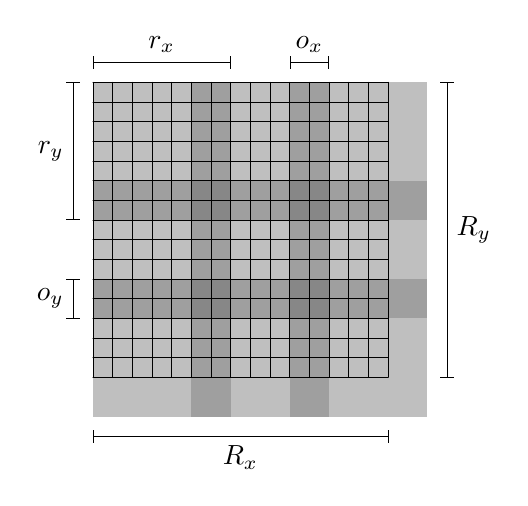
\begin{tikzpicture}[scale = 0.25, very thin]
	
		% Tiles
		\foreach \x in {0,...,2} {
			\foreach \y in {0,...,2}{
				\fill[gray, opacity = 0.5] (\x * 5, -\y * 5) rectangle ++(7, -7);
			}
		}
		
		% Grid
		\draw[step = 1 cm, cap = round] (0, 0) grid (15, -15);
		
		% Markers
		\draw[|-|] (0, -18) -- node[below]	{$R_x$} ++(15, 0);
		\draw[|-|] (18, 0) -- node[right]	{$R_y$} ++(0, -15);
		\draw[|-|] (0, 1) 	-- node[above]	{$r_x$} ++(7, 0);
		\draw[|-|] (-1, 0) 	-- node[left]	{$r_y$} ++(0, -7);
		\draw[|-|] (10, 1) 	-- node[above]	{$o_x$} ++(2, 0);
		\draw[|-|] (-1, -10) -- node[left]	{$o_y$} ++(0, -2);
	
	\end{tikzpicture}
\end{document}

		\caption{}
		\label{fig:tiling_layout}
	\end{subfigure}%
	\begin{subfigure}{0.5\textwidth}
		\centering
		\documentclass{standalone}
\usepackage{calc}
\usepackage{tikz}

\begin{document}
	\begin{tikzpicture}[scale = 0.25, very thin]
	
		% Tiles
%		\foreach \x in {0,...,2} {
%			\foreach \y in {0,...,2}{
%				\fill[gray, opacity = 0.5] (\x * 5, -\y * 5) rectangle ++(7, -7);
%			}
%		}

		% Summed up masks
		\node [anchor = north west, inner sep = 0] at (0, 0) {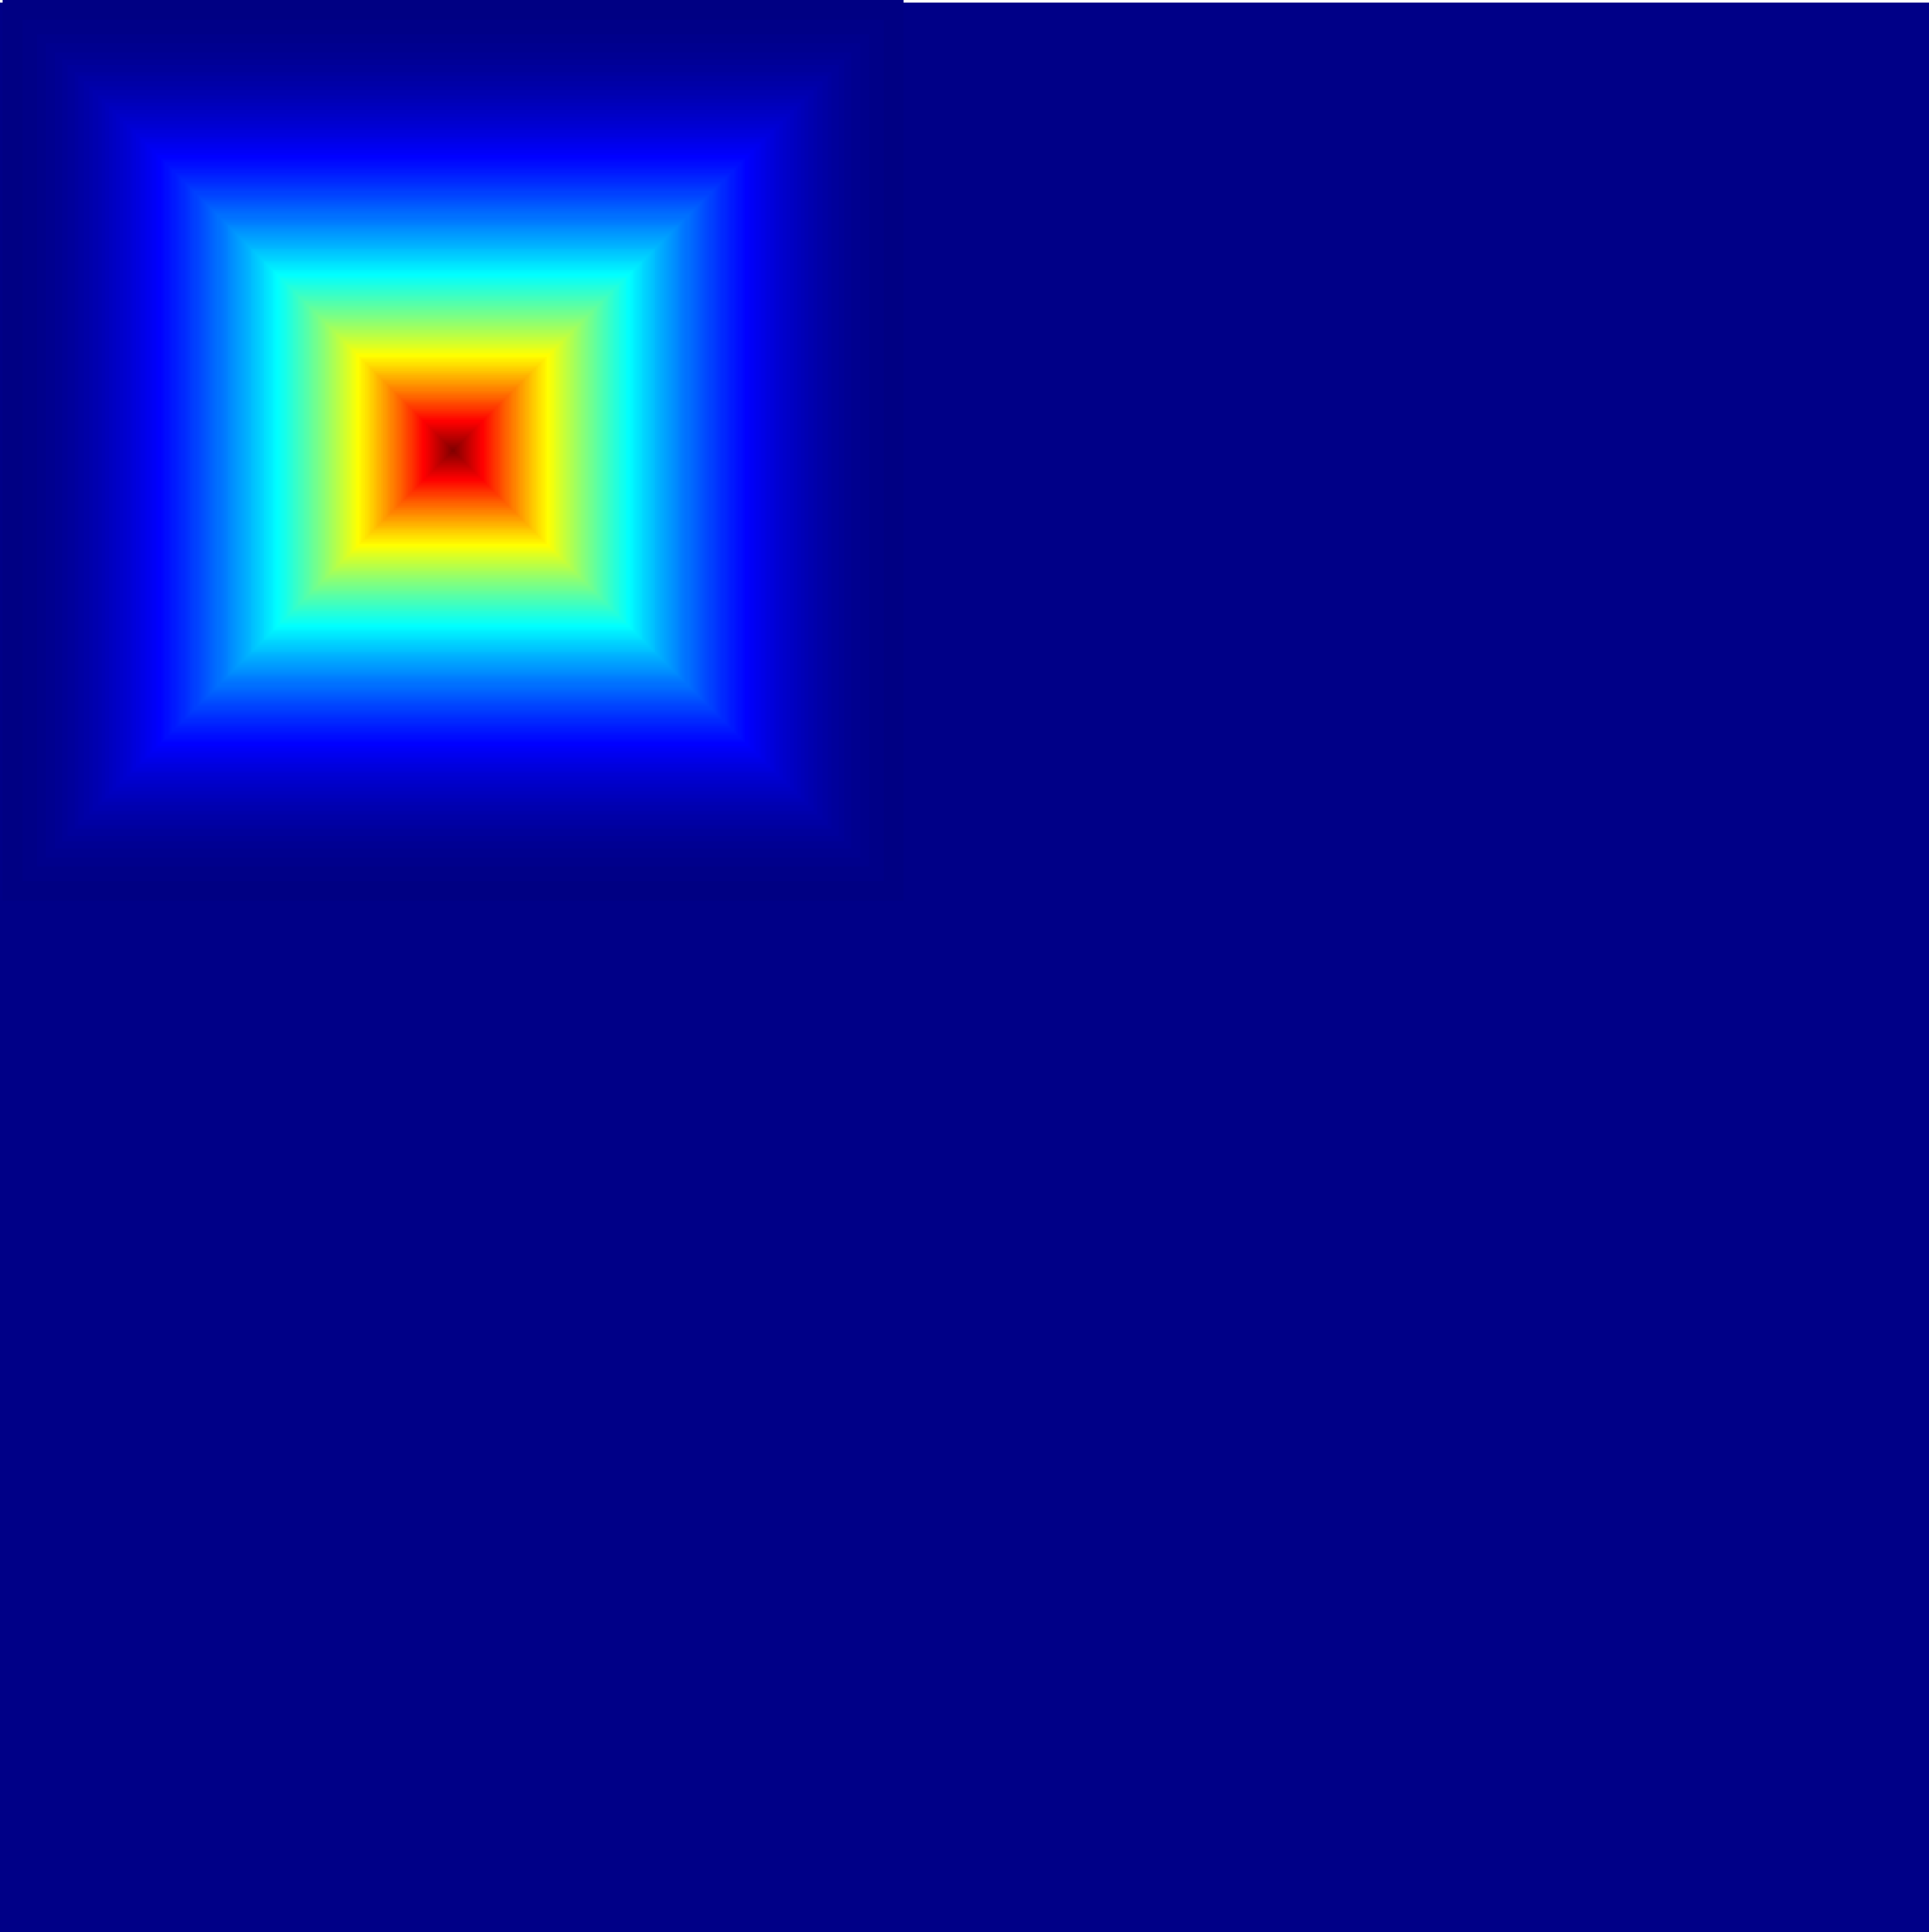
\includegraphics[width = 3.75cm]{./figures/tiling/mask1}};
		\node [anchor = east, scale=2] at (-0.5, -3.6) {$\ast$};
		% Grid
%		\draw[step = 1 cm, cap = round] (0, 0) grid (15, -15);
		
		% Invisible markers for accurate placement in figure 
		\begin{scope}[opacity = 0]
			\draw[|-|] (0, -18) -- node[below]	{$R_x$} ++(15, 0);
%			\draw[|-|] (18, 0) -- node[right]	{$R_y$} ++(0, -15);
			\draw[|-|] (0, 1) 	-- node[above]	{$r_x$} ++(7, 0);
%			\draw[|-|] (-1, 0) 	-- node[left]	{$r_y$} ++(0, -7);
			\draw[|-|] (10, 1) 	-- node[above]	{$o_x$} ++(2, 0);
%			\draw[|-|] (-1, -10) -- node[left]	{$o_y$} ++(0, -2);
		\end{scope}
		
	\end{tikzpicture}
\end{document}
		\caption{}
		\label{fig:sum_of_quadratic_blending_masks}
	\end{subfigure}%
	\caption[Tiling layout]
			{(a) Layout of the tiles that cover the attenuation layers.
				 The pixel grid of size $R_x \times R_y$ is covered by tiles of $r_x \times r_y$ pixels with an overlap of $o_x$ in horizontal and $o_y$ in vertical direction.
			 (b) The sum of the per-tile quadratic blending masks used for the normalization.}
\end{figure}
The inputs for the tiling algorithm are the resolution of the tiles $r = (r_x, r_y)$ and the overlap in horizontal and vertical direction, $o = (o_x, o_y)$. 
The tiles are then laid out in a grid beginning in the top left corner of the layer. 
The number of tiles needed to cover the plane can be calculated by 
\begin{equation}
	N_x = \left \lceil \dfrac{R_x - o_x}{r_x - o_x} \right \rceil
	\qquad 
	\text{and} 
	\qquad
	N_y = \left \lceil \dfrac{R_y - o_y}{r_y - o_y} \right \rceil.
\end{equation}
The combination of the same tile from each layer forms a subsection of the original layer stack and so, essentially a new attenuator of smaller size and lower resolution.
The optimization is then performed on all of the subsections with a smaller propagation matrix per tile (fewer columns). 
As a consequence, less memory is used to store attenuation layers and propagation data in each step.
In the end, the optimized tiles are put together to form the complete attenuation layers. 

In general, the borders of the attenuator contain less ray-propagation information and thus provide fewer constraints for the optimization. 
This introduces artifacts that are clearly visible in the reassembled layers as shown in figure~\ref{fig:comparison_tile_overlap_vs_no_overlap}.
\begin{figure}[tb]
	\centering
	\begin{subfigure}{0.23\textwidth}
		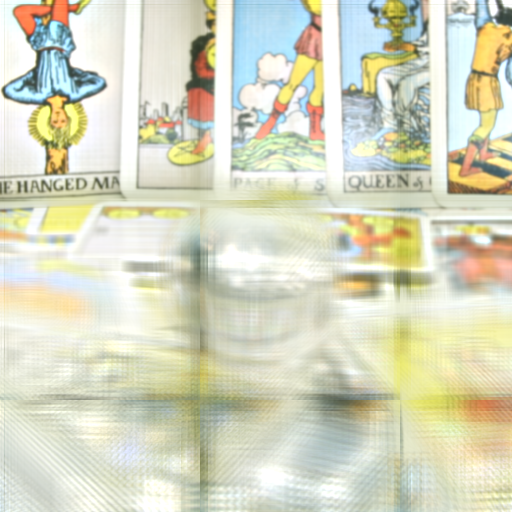
\includegraphics[width = \textwidth]{../Figures/tiling/tarot_tiles3x3x200x200_no_overlap_3_layers/1.png}
		
		\vspace{0.15cm}
		
		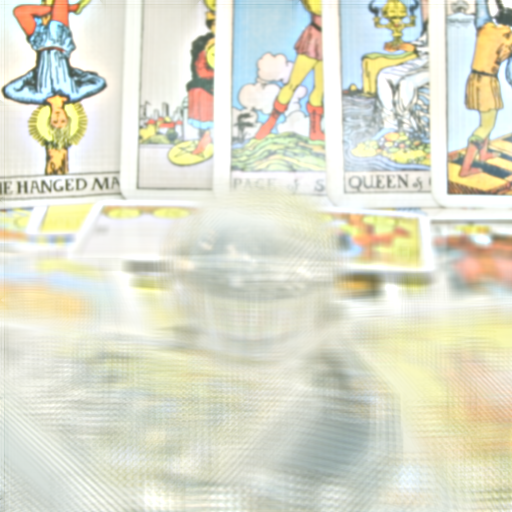
\includegraphics[width = \textwidth]{../Figures/tiling/tarot_tiles5x5x200x200_overlap0.5_3_layers/1.png}
		\caption{Layer 1}
	\end{subfigure}\hspace{0.15cm}%
	\begin{subfigure}{0.23\textwidth}
		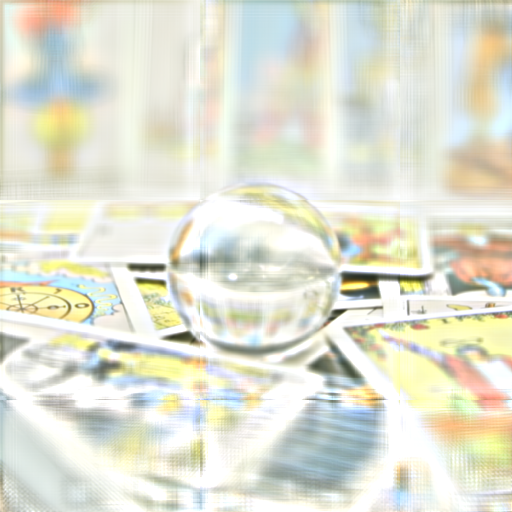
\includegraphics[width = \textwidth]{../Figures/tiling/tarot_tiles3x3x200x200_no_overlap_3_layers/2.png}
		
		\vspace{0.15cm}
		
		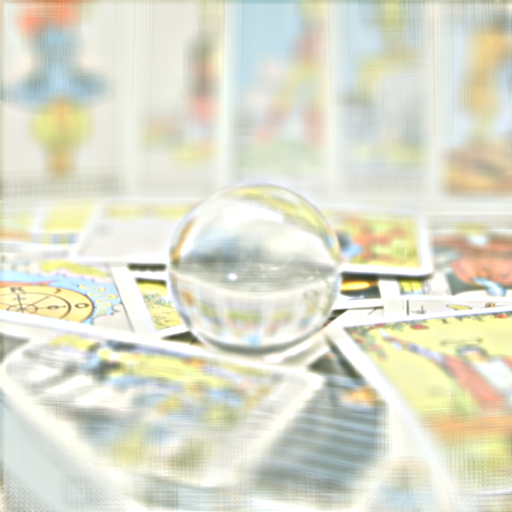
\includegraphics[width = \textwidth]{../Figures/tiling/tarot_tiles5x5x200x200_overlap0.5_3_layers/2.png}
		\caption{Layer 2}
	\end{subfigure}\hspace{0.15cm}%
	\begin{subfigure}{0.23\textwidth}
		
\includegraphics[width = \textwidth]{../Figures/tiling/tarot_tiles3x3x200x200_no_overlap_3_layers/3.png}
		
		\vspace{0.15cm}
		
		
\includegraphics[width = \textwidth]{../Figures/tiling/tarot_tiles5x5x200x200_overlap0.5_3_layers/3.png}
		\caption{Layer 3}
	\end{subfigure}\hspace{0.15cm}%
	\begin{subfigure}{0.23\textwidth}
		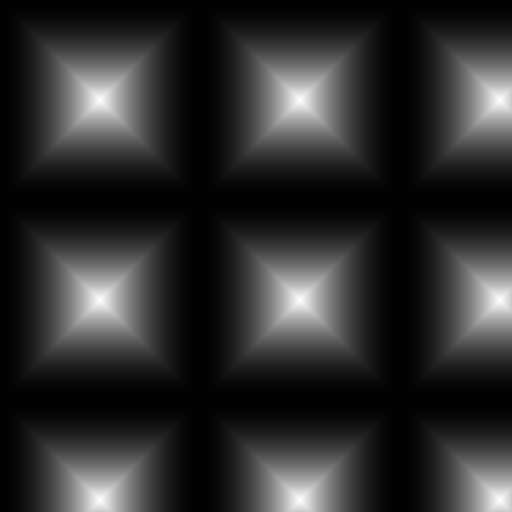
\includegraphics[width = \textwidth]{../Figures/tiling/tarot_tiles3x3x200x200_no_overlap_3_layers/blendingMaskSum.png}
		
		\vspace{0.15cm}
		
		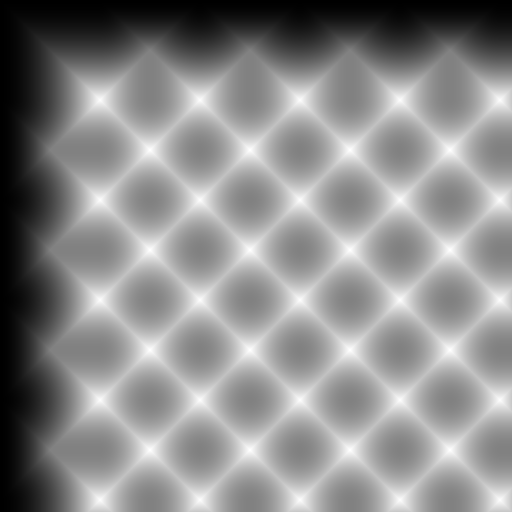
\includegraphics[width = \textwidth]{../Figures/tiling/tarot_tiles5x5x200x200_overlap0.5_3_layers/blendingMaskSum.png}
		\caption{Blending masks}
	\end{subfigure}%
	\caption[Impact of tile overlap on attenuation layers]
			{Impact of tile overlap on attenuation layers.
			 Top: Tiles have no overlap and grid artifacts are visible.
			 Bottom: With a 50\% overlap, the artifacts are no longer noticeable, but more tiles are needed.}
	\label{fig:comparison_tile_overlap_vs_no_overlap}
\end{figure} 
To solve this issue, the tiles have to overlap. 
In this case, when reassembling the layers from the tiles, the overlaps need to be blended with a mask:
After the optimization, each tile gets multiplied with a quadratic blending mask.
The finished layers are then obtained by summing the tiles and dividing by the sum of the blending masks shown in figure~\ref{fig:sum_of_quadratic_blending_masks}.
For the results shown in this work, a quadratic blending mask was used (weights increase quadratically towards the middle of the tile).

\section{Performance of SART}
\label{sec:performance_of_SART}

The two iterative solvers described in section~\ref{sec:iterative_reconstruction} are compared in figure~\ref{fig:sart_vs_lsqlin} in terms of reconstruction error and runtime.
\begin{figure}[tb]
	\begin{subfigure}{0.5\textwidth}
		\centering
		\documentclass{standalone}
\usepackage{pgfplots}

\begin{document}
	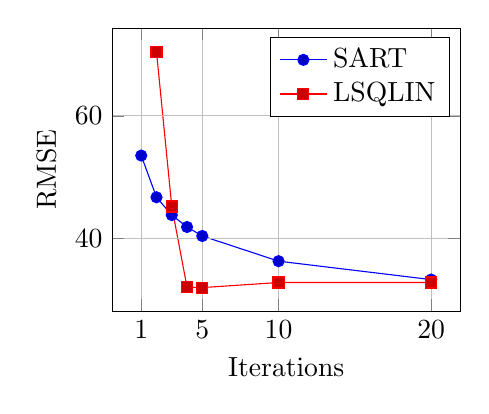
\begin{tikzpicture}
		
		\begin{axis}[	legend pos = north east, 
						legend cell align = left,
						xtick = {1, 5, 10, 20},
						ylabel = {RMSE},
						xlabel = {Iterations},
						ylabel near ticks,
						grid = major,
						axis on top = true,
						width = 6 cm]
		
			\addplot coordinates {
				(1, 53.517116)
				(2, 46.6983)
				(3, 43.7923)
				(4, 41.8413)
				(5, 40.3709)
				(10, 36.2524)
				(20, 33.2420)
			};
			\addlegendentry{SART};
			
			\addplot coordinates {
				(2, 70.477447)
				(3, 45.188843)
				(4, 32.001308)
				(5, 31.934515)
				(10, 32.764468)
				(20, 32.766828)
			};
			\addlegendentry{LSQLIN};
			
			 
		\end{axis}
		
	\end{tikzpicture}
\end{document}
		\caption{}
		\label{fig:sart_lsqlin_iterations_vs_rmse}
	\end{subfigure}%
	\begin{subfigure}{0.5\textwidth}
		\centering
		\documentclass{standalone}
\usepackage{pgfplots}

\begin{document}
	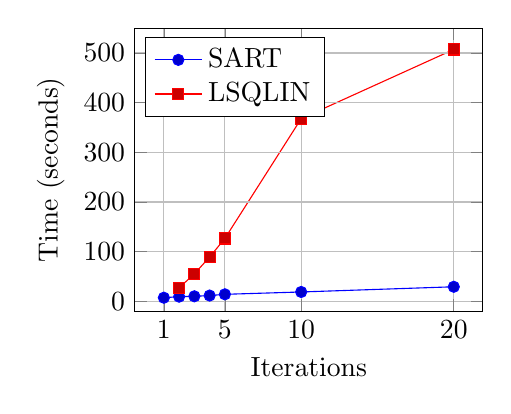
\begin{tikzpicture}
		
		\begin{axis}[	legend pos = north west, 
						legend cell align = left,
						ymin = -20,
						ymax = 550,
						xtick = {1, 5, 10, 20},
						ytick = {0, 100, 200, 300, 400, 500},
						ylabel = {Time (seconds)},
						xlabel = {Iterations},
						ylabel near ticks,
						grid,
						axis on top = true,
						width = 6 cm]
		
			\addplot coordinates {
				(1, 7.0933)
				(2, 9.2096)
				(3, 9.9564)
				(4, 11.4550)
				(5, 13.9412)
				(10, 18.6697)
				(20, 29.1313)
			};
			\addlegendentry{SART};
			
			\addplot coordinates {
				(2, 26.9930)
				(3, 55.2522)
				(4, 89.0784)
				(5, 126.5243)
				(10, 367.7888)
				(20, 507.2163)
			};
			\addlegendentry{LSQLIN};
			
			 
		\end{axis}
		
	\end{tikzpicture}
\end{document}
		\caption{}
		\label{fig:sart_lsqlin_iterations_vs_time}
	\end{subfigure}%
	\caption[Performance assessment of the optimization]
			{Performance assessment of the optimization.
			 The two iterative methods \mbox{SART} and \mbox{MATLAB's} linear least squares solver LSQLIN are compared in terms of \mbox{RMSE} (a) and runtime (b).
			 The input light field is the same as in figure~\ref{fig:baseline_scaling} and five attenuation layers were used.}
	\label{fig:sart_vs_lsqlin}
\end{figure}
Although the standard least squares solver uses fewer iterations compared to SART, the computation time is significantly longer.
For the specific experiment in the figure, both methods achieve the same RMSE with twenty iterations, but SART performs the twenty iterations in the same time as LSQLIN solves two iterations.
Furthermore, the simple update rule of SART allows for concurrent optimization in each color channel as opposed to LSQLIN, which needs to be run on every channel separately.
This shows that SART is a superior solver for this large scale layered 3D problem.

Next, the reconstruction quality of SART is compared against the number of layers used to display.
Adding more layers means adding more pixels and hence there are more degrees of freedom for the optimization.
In theory the more layers there are, the closer is the display to a full attenuation volume.
The plot in figure~\ref{fig:sart_layers_vs_psnr} shows how the PSNR of the simulated projections behaves with with up to twenty layers.
\begin{figure}[tb]
	\begin{subfigure}{\textwidth}
		\centering
		\documentclass{standalone}
\usepackage{pgfplots}

\begin{document}
	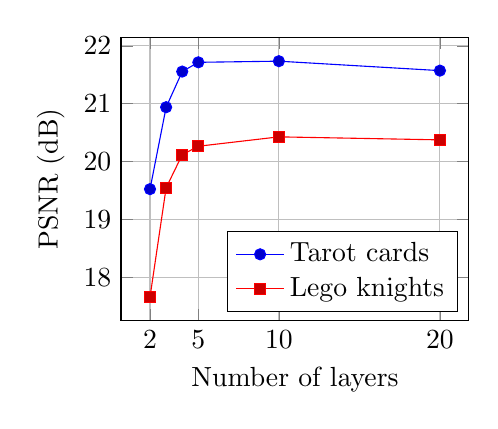
\begin{tikzpicture}
		
		\begin{axis}[	legend pos = south east, 
						legend cell align = left,
						xtick = {2, 5, 10, 20},
						ytick = {18, 19, 20, 21, 22},
						ylabel = {PSNR (dB)},
						xlabel = {Number of layers},
						ylabel near ticks,
						grid,
						axis on top = false,
						width = 6 cm]
						
		%% NOTE: I added the 4.7712 = 10 * log_10(3) because I forgot to normalize the MSE by the number of color channels 
		
			\addplot coordinates {
				(2, 14.7555 + 4.7712)
				(3, 16.1691 + 4.7712)
				(4, 16.7842 + 4.7712)
				(5, 16.9441 + 4.7712)
				(10, 16.9636 + 4.7712)
				(20, 16.8005 + 4.7712)
			};
			\addlegendentry{Tarot cards};
			
			\addplot coordinates {
				(2, 12.8945 + 4.7712)
				(3, 14.7783 + 4.7712)
				(4, 15.3490 + 4.7712)
				(5, 15.4956 + 4.7712)
				(10, 15.6576 + 4.7712)
				(20, 15.6058 + 4.7712)
			};
			\addlegendentry{Lego knights};
			
			 
		\end{axis}
		
	\end{tikzpicture}
\end{document}
	\end{subfigure}%
	\caption[Impact of layer count on \mbox{PSNR}]
			{Impact of layer count on the \mbox{PSNR}.
			 Performance comparison of the attenuation display for two different scenes from the Stanford light field archive.
			 Ten iterations of SART were performed for each scene.}
	\label{fig:sart_layers_vs_psnr}
\end{figure}

\section{Contrast Sensitivity}

The contrast sensitivity is a very important measure for human visual perception.
The human visual system does not only perceive light intensity in a non-linear fashion, but it is also very sensitive to contrast.
Contrast sensitivity is defined to be the threshold at which the individual can no longer distinguish between contrast differences, and this threshold changes with spatial frequency.
The top left image in figure~\ref{fig:contrast_sensitivity} shows the contrast sensitivity pattern which changes horizontally in frequency and vertically in contrast.
\begin{figure}[tb]
	\begin{subfigure}{0.45\textwidth}
		\documentclass{standalone}
\usepackage{pgfplots}
\usepgfplotslibrary{groupplots}
\usetikzlibrary{matrix, positioning}
\pgfplotsset{compat=newest}

\begin{document}
	\begin{tikzpicture}
	    \begin{groupplot}
	    [group style = {group name = my plots, group size = 1 by 1, vertical sep = 0.15cm, 
				    	every plot/.style = {
				    		axis equal image,
				    		axis lines = left, 
							hide axis, 
							xtick=\empty, 
							ytick=\empty, 
				    	}}, 
		    height = 5.5cm
		]
				
			\nextgroupplot[	colorbar, 
							colormap/blackwhite, 
							point meta min = 0, 
							point meta max = 1,
							colorbar style = {
								ytick = {0, 1},
								every tick label/.append style = {font = \small},
								shift = {(-2mm, 0cm)}, 
								width = 2mm
							}]
				
				\addplot graphics[xmin=0, xmax=640, ymin=0, ymax=480] {../Figures/contrast/contrast_sensitivity.png};
	    
	    \end{groupplot}
	    
	    \node[below = 0.3cm of my plots c1r1.south] {Contrast sensitivity pattern};
	    
	    
	\end{tikzpicture}
\end{document}
	\end{subfigure}\hfill%
	\begin{subfigure}{0.45\textwidth}
		\documentclass{standalone}
\usepackage{pgfplots}
\usepgfplotslibrary{groupplots}
\usetikzlibrary{matrix, positioning}
\pgfplotsset{compat=newest}

\begin{document}
	\begin{tikzpicture}
	    \begin{groupplot}
	    [group style = {group name = my plots, group size = 1 by 2, vertical sep = 0.15cm, 
				    	every plot/.style = {
				    		axis equal image,
				    		axis lines = left, 
							hide axis, 
							xtick=\empty, 
							ytick=\empty, 
				    	}}, 
		    height = 5.5cm
		]
			
			\nextgroupplot[	colorbar, 
							colormap/blackwhite, 
							point meta min = 0, 
							point meta max = 1,
							colorbar style = {
								ytick = {0, 1},
								every tick label/.append style = {font = \small},
								shift = {(-2mm, 0cm)}, 
								width = 2mm,
								opacity = 0
							}]
							
				\addplot graphics[xmin=0, xmax=320, ymin=0, ymax=120] {../Figures/contrast/2layer_1x_resolution/2layer_1x_resolution_rec.png};
				\coordinate (top) at (rel axis cs:0,1);% coordinate at top of the first plot
				
			\nextgroupplot[	colorbar, 
							colormap/jet, 
							point meta min = 0, 
							point meta max = 0.2,
							colorbar style = {
								ytick = {0, 0.2},
								every tick label/.append style = {font = \small},
								shift = {(-2mm, 0cm)}, 
								width = 2mm
							}]
				
				\addplot graphics[xmin=0, xmax=320, ymin=0, ymax=120] {../Figures/contrast/2layer_1x_resolution/2layer_1x_resolution.png};
	    
	    \end{groupplot}
	    
	    \node[below = 0.15cm of my plots c1r2.south] {2 layers};
	    
	    
	\end{tikzpicture}
\end{document}
	\end{subfigure}%
	\\
	\begin{subfigure}{0.45\textwidth}
		\documentclass{standalone}
\usepackage{pgfplots}
\usepgfplotslibrary{groupplots}
\usetikzlibrary{matrix, positioning}
\pgfplotsset{compat=newest}

\begin{document}
	\begin{tikzpicture}
	    \begin{groupplot}
	    [group style = {group name = my plots, group size = 1 by 2, vertical sep = 0.15cm, 
				    	every plot/.style = {
				    		axis equal image,
				    		axis lines = left, 
							hide axis, 
							xtick=\empty, 
							ytick=\empty, 
				    	}}, 
		    height = 5.5cm
		]
			
			\nextgroupplot
							
				\addplot graphics[xmin=0, xmax=320, ymin=0, ymax=120] {../Figures/contrast/2layer_2x_resolution/2layer_2x_resolution_rec.png};
				\coordinate (top) at (rel axis cs:0,1);% coordinate at top of the first plot
				
			\nextgroupplot[	colorbar, 
							colormap/jet, 
							point meta min = 0, 
							point meta max = 0.2,
							colorbar style = {
								ytick = {0, 0.2},
								every tick label/.append style = {font = \small},
								shift = {(-2mm, 0cm)}, 
								width = 2mm
							}]
				
				\addplot graphics[xmin=0, xmax=320, ymin=0, ymax=120] {../Figures/contrast/2layer_2x_resolution/2layer_2x_resolution.png};
	    
	    \end{groupplot}
	    
	    \node[below = 0.15cm of my plots c1r2.south] {2 layers, 2x resolution};
	    
	    
	\end{tikzpicture}
\end{document}
	\end{subfigure}\hfill%
	\begin{subfigure}{0.45\textwidth}
		\documentclass{standalone}
\usepackage{pgfplots}
\usepgfplotslibrary{groupplots}
\usetikzlibrary{matrix, positioning}
\pgfplotsset{compat=newest}

\begin{document}
	\begin{tikzpicture}
	    \begin{groupplot}
	    [group style = {group name = my plots, group size = 1 by 2, vertical sep = 0.15cm, 
				    	every plot/.style = {
				    		axis equal image,
				    		axis lines = left, 
							hide axis, 
							xtick=\empty, 
							ytick=\empty, 
				    	}}, 
		    height = 5.5cm
		]
			
			\nextgroupplot
							
				\addplot graphics[xmin=0, xmax=320, ymin=0, ymax=120] {../Figures/contrast/5layer_1x_resolution/5layer_1x_resolution_rec.png};
				\coordinate (top) at (rel axis cs:0,1);% coordinate at top of the first plot
				
			\nextgroupplot[	colorbar, 
							colormap/jet, 
							point meta min = 0, 
							point meta max = 0.2,
							colorbar style = {
								ytick = {0, 0.2},
								every tick label/.append style = {font = \small},
								shift = {(-2mm, 0cm)}, 
								width = 2mm
							}]
				
				\addplot graphics[xmin=0, xmax=320, ymin=0, ymax=120] {../Figures/contrast/5layer_1x_resolution/5layer_1x_resolution.png};
	    
	    \end{groupplot}
	    
	    \node[below = 0.15cm of my plots c1r2.south] {5 layers};
	    
	    
	\end{tikzpicture}
\end{document}
	\end{subfigure}%
	\\
	\begin{subfigure}{0.45\textwidth}
		\documentclass{standalone}
\usepackage{pgfplots}
\usepgfplotslibrary{groupplots}
\usetikzlibrary{matrix, positioning}
\pgfplotsset{compat=newest}

\begin{document}
	\begin{tikzpicture}
	    \begin{groupplot}
	    [group style = {group name = my plots, group size = 1 by 2, vertical sep = 0.15cm, 
				    	every plot/.style = {
				    		axis equal image,
				    		axis lines = left, 
							hide axis, 
							xtick=\empty, 
							ytick=\empty, 
				    	}}, 
		    height = 5.5cm
		]
			
			\nextgroupplot
							
				\addplot graphics[xmin=0, xmax=320, ymin=0, ymax=120] {../Figures/contrast/5layer_2x_resolution/5layer_2x_resolution_rec.png};
				\coordinate (top) at (rel axis cs:0,1);% coordinate at top of the first plot
				
			\nextgroupplot[	colorbar, 
							colormap/jet, 
							point meta min = 0, 
							point meta max = 0.2,
							colorbar style = {
								ytick = {0, 0.2},
								every tick label/.append style = {font = \small},
								shift = {(-2mm, 0cm)}, 
								width = 2mm
							}]
				
				\addplot graphics[xmin=0, xmax=320, ymin=0, ymax=120] {../Figures/contrast/5layer_2x_resolution/5layer_2x_resolution.png};
	    
	    \end{groupplot}
	    
	    \node[below = 0.15cm of my plots c1r2.south] {5 layers, 2x resolution};
	    
	    
	\end{tikzpicture}
\end{document}
	\end{subfigure}\hfill%
	\begin{subfigure}{0.45\textwidth}
		\documentclass{standalone}
\usepackage{pgfplots}
\usepgfplotslibrary{groupplots}
\usetikzlibrary{matrix, positioning}
\pgfplotsset{compat=newest}

\begin{document}
	\begin{tikzpicture}
	    \begin{groupplot}
	    [group style = {group name = my plots, group size = 1 by 2, vertical sep = 0.15cm, 
				    	every plot/.style = {
				    		axis equal image,
				    		axis lines = left, 
							hide axis, 
							xtick=\empty, 
							ytick=\empty, 
				    	}}, 
		    height = 5.5cm
		]
			
			\nextgroupplot
							
				\addplot graphics[xmin=0, xmax=320, ymin=0, ymax=120] {../Figures/contrast/5layer_3x_resolution/5layer_3x_resolution_rec.png};
				\coordinate (top) at (rel axis cs:0,1);% coordinate at top of the first plot
				
			\nextgroupplot[	colorbar, 
							colormap/jet, 
							point meta min = 0, 
							point meta max = 0.2,
							colorbar style = {
								ytick = {0, 0.2},
								every tick label/.append style = {font = \small},
								shift = {(-2mm, 0cm)}, 
								width = 2mm
							}]
				
				\addplot graphics[xmin=0, xmax=320, ymin=0, ymax=120] {../Figures/contrast/5layer_3x_resolution/5layer_3x_resolution.png};
	    
	    \end{groupplot}
	    
	    \node[below = 0.15cm of my plots c1r2.south] {5 layers, 3x resolution};
	    
	    
	\end{tikzpicture}
\end{document}
	\end{subfigure}%
	\caption[Contrast sensitivity analysis for layered 3D displays]
			{Contrast sensitivity analysis for layered 3D displays.
			 Shown are the simulated display projection from a viewing direction perpendicular to the display (top) and the absolute error (bottom) for a two-layer and five-layer display with different layer resolution.
			 The light field is constant in angle, contains increasing spatial frequency from left to right and increasing contrast from top to bottom.}
	\label{fig:contrast_sensitivity}
\end{figure}
In context of Layered 3D, it is of course desirable that the loss of contrast in the emitted images is as little as possible.
The experiments in figure~\ref{fig:contrast_sensitivity} quantify the absolute error of contrast with a light field comprising the contrast sensitivity pattern in spatial dimension which is constant in angular dimension.
It shows that adding more layers reduces the magnitude of the error, and increasing the layer resolution reduces the error for higher frequencies.

\section{Graphical User Interface}
\label{sec:GUI}

All functionalities of the pipeline are made available through a graphical user interface \mbox{(GUI)} for ease of use.
The main window is shown in figure~\ref{fig:gui_overview} for a particular use case.
\begin{figure}[tb]
	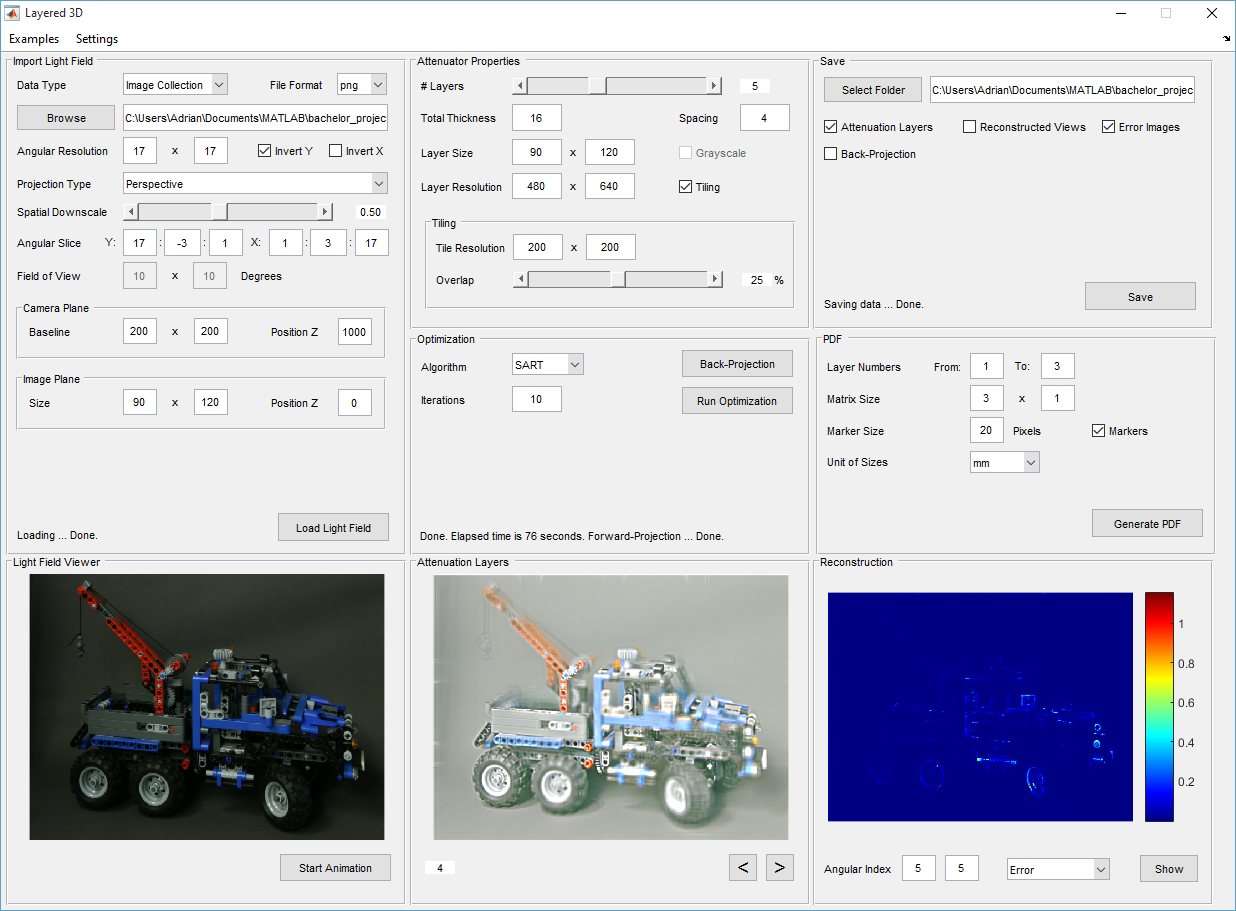
\includegraphics[width = \linewidth]{../Figures/gui/overview}
	\caption[Graphical user interface]
			{Graphical user interface for the \emph{Layered 3D} software developed with MATLAB.}
	\label{fig:gui_overview}
\end{figure}
A typical workflow involves three main steps, which correspond to the three columns in the window.
In the first step, the user imports a light field from either a folder of images or a \mbox{Lytro} container file.
The user can specify the projection type, camera- and image plane parameters as well as spatial- and angular downsampling in case memory is scarce.
After a successful import, the individual angular views are displayed in the preview window below.
The seconds step involves the configuration of the attenuator where the user enters the desired display thickness, size and resolution.
Before running the optimization, the user has the option to back-project the light field in case he/she want to ensure that the light fields depth range is aligned with the display.
In the last step, after optimization has completed, the user can preview the results (attenuation layers, reconstructed views or error images) in the window below or save them to disk.
Finally, a \mbox{PDF} file with the attenuation masks can be generated, ready to print on transparencies.

The software together with the GUI is available as an executable\footnote{The software available at \url{https://github.com/awaelchli/bachelor_project}.} 
and does not require a \mbox{MATLAB} installation in order to run.

\section{Benefits and Limitations}
\label{sec:benefits_limitations}

From a theoretical standpoint, the layered 3D architecture seems to be very promising.
The analysis shows that multiplicative displays encompass extended spectral support resulting in a higher depth of field compared to other automultiscopic systems.
The multi-layer design eliminates the trade-off between angular- and spatial resolution that is present with parallax barriers or integral imaging.
In practice, there are a few limitations that need to be addressed.
First off, to solve the multiplicative problem given by equation~\ref{eq:transmittance_layers} it is assumed that the transmission values are positive in order to solve the problem in a linear manner with the logarithm applied.
For the physical realization, this is of course a well justified assumption since negative transmission is not possible to achieve.
Nonetheless, the restriction to positive transmittance is reducing the space of solutions for optimal attenuation layers.
Although it would require an entirely different approach, it is plausible to achieve better results if real valued transmission values were permitted.

The prototypes produced in the context of this thesis are suited for demonstration purposes, though the viewing angles are limited to a small range.
Unfortunately, experiments to show objects in virtual planes outside the displays enclosure were not successful.
Another challenge with display fabrication is the manual layer alignment.
The marks printed on the border of the layers help with alignment, but the process remains tedious and becomes increasingly harder with more layers.
Moreover, there are no universally best printer settings (amount of ink, drying time etc.) for printing on transparencies.
The settings have to be tuned by trial-and-error depending on the particular printer model and transparencies.
Also, Moir\'{e} does not seem to be a problem because of the natural blending of ink.

\section{Improvements and Future Work}
\label{sec:future_work}

The current implementation in MATLAB provides the necessary features in order to produce a static layered 3D display.
However, with greater effort a lot of operations can be made more efficient.
A GPU implementation of SART like the one from \cite{SARTGPU} could be incorporated in the software to accelerate the optimization process.
A parallelization of SART is possible because the update rule depends solely on matrix multiplication and addition.
The parallel approach would also eliminate the need of explicitly pre-computing the propagation matrix, which is a computationally- and memory intensive process.
Still, the final printing and layer alignment remains time consuming and must be attacked with patience.
Alternatively the masks could be printed directly on glass which would result in a higher build quality and precise layer alignment.

Some assumptions that are incorporated into the software could be generalized.
Among them is the pinhole camera model that could be extended to a more realistic lens model.
Further, only regularly sampled light fields are supported which would make it harder to adopt light fields from unconventional capturing devices.

As \cite{WetzsteinTensor} have shown, LCD panels can be used to modulate light instead of printed layers.
The benefit here is that the panels can be accurately aligned and calibrated once, and no further adjustments to the hardware are necessary in order to view different content.
Building the display however requires advanced technical knowledge in developing custom electronics to control and interface with the panels.